%about objects not information; we can discuss in outside the box the issue of
%information needed forver but shuttled in and out.

\chapter{Extreme Scalability of Long-lived Data}
\label{chapter:large-long-lived}

All of the tuning advice presented so far in this book can only get you so far.
Sometimes, despite your best efforst of tuning entities and collections, your
application's objects still do not fit into the memory constraints of the target
platform. Managing a great number of long-lived objects therefore comes with its
own set of challenges, even though objects these objects are free from the bugs
that riddle those with correlated lifetime. To manage objects that, after a
reasonable amount of tuning, still don't fit into the heap, you have three
solutions at your disposal: throw hardware at the problem, implement a kind of
demand paging, or code your data models in a non-object oriented way.

\paragraph{Buy More Memory} The first solution you may consider is buying more
memory for the target platform. If your budget allows for this, then by all means
you should strongly consider doing so. There are some downsides to keep in mind.
The first is heap size limits. At some point, you will need to switch from a
32-bit JVM to a 64-bit JVM\index{64-bit}. This switch will result in a large
increase in overhead. As discussed earlier, the amount of blowup resulting from a
switch to a 64-bit JVM depends on the degree of delegation in your data models. A
64-bit JVM only adds overhead to the extent that your data models have headers
and pointers. The alternative, running with compressed
references\index{Compressed References}, limits you to around 32GB of memory, and
imposes a few percent slowdown. In addition, running with a large heap can result
in increases in the length and fluctuations in pause times.

\paragraph{Shuttle Objects in and Out of the Java Heap} Rather than attempting to
fit all of your objects into a single heap, you can store them outside of the
Java heap, and swap them in (and out), on demand. If the logic of your
application allows for recomputing the data stored in these objects, you need to
be careful to compare the recreation cost with the costs of marshalling objects.
You can choose to marshall objects to and from a local disk, or you can use one
of several frameworks that provide a distributed key-value map.

\paragraph{Break the Java Mold} Despite being an object-oriented language, there
is nothing in the Java language that prevents you from storing objects in a
non-object oriented way --- nothing, that is, except programming time and
maintenance expense. It is possible to store data only in arrays, as one would in
a language such as Fortran, and retain a great deal of object orientation in your
data models and programming interfaces. 

This chapter presents a methodology for predicting the scalability of your data
models, and presents several solutions to demand-marshalling objects, and for
storing objects in a ``Fortran style''.

\section{Scalability: Quantitative Methodology}

\begin{figure}
\centering
	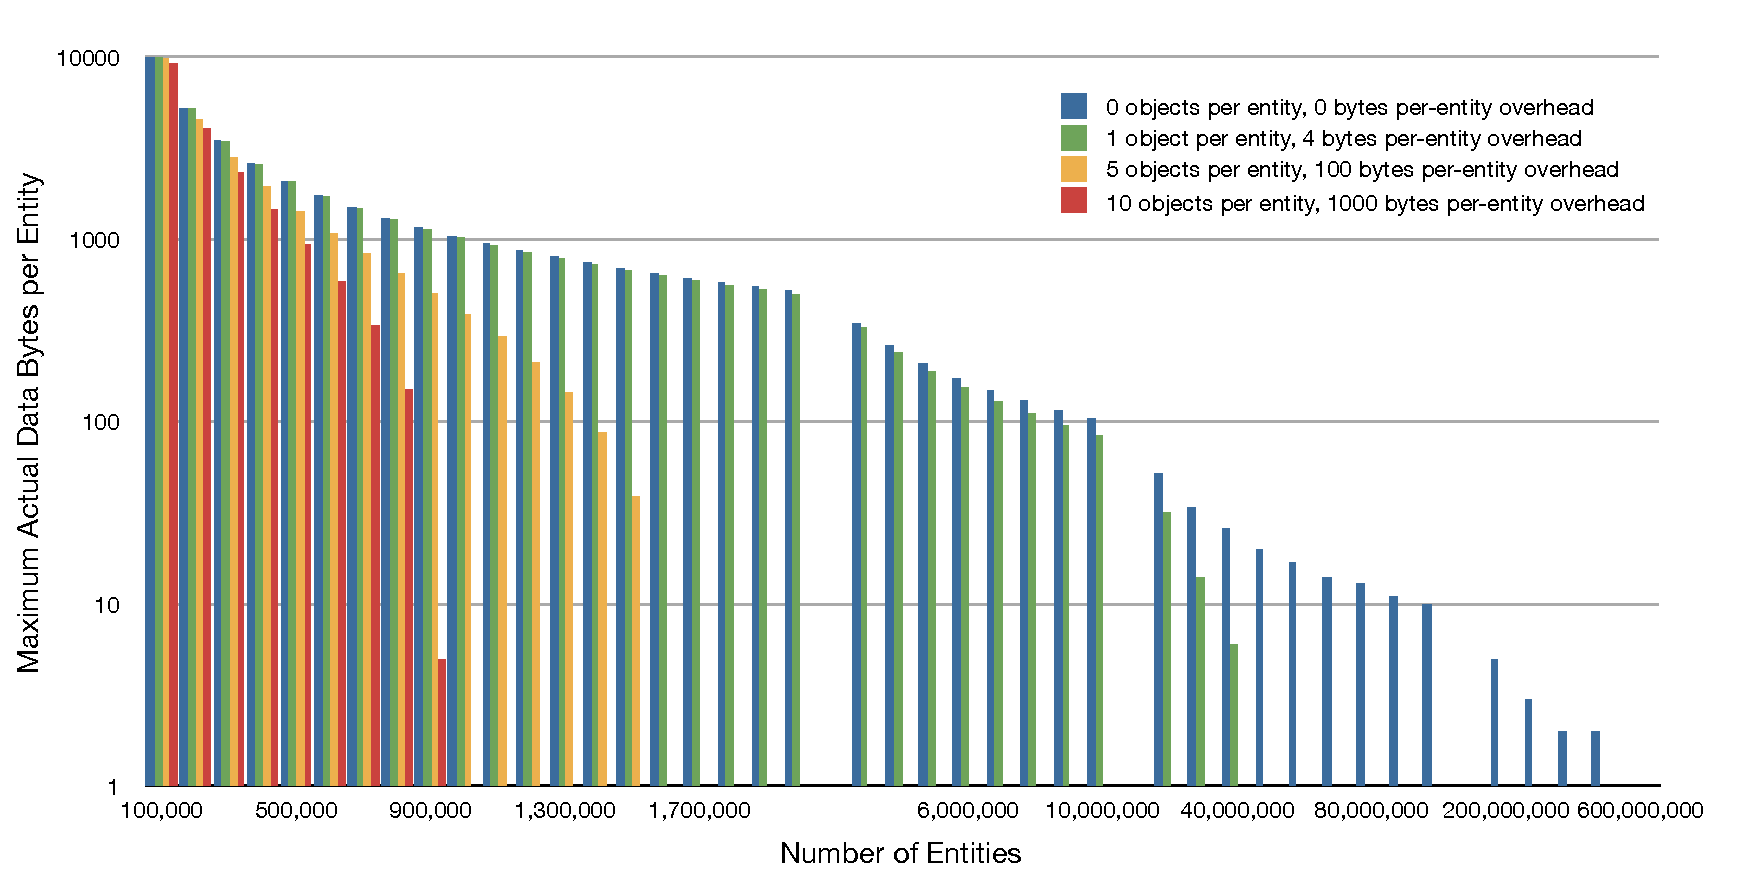
\includegraphics[width=\textwidth]{part4/Figures/maxActualData}
	\caption{The amount of actual data you can store in your entities depends on
	the degree of delegation in your entities, and the per-entry overhead of the collection in which these entities
	reside. This chart assumes a limit of 1 gigabyte of Java heap.}
	\label{fig:maxActualData}
\end{figure}

TODO: write this section, explaining \autoref{fig:maxActualData}.

\section{Representing Relationships}

When representing relationships between entities, using standard object oriented
practices, you are severely limited in the number of entities and relationships
that you can store. Doing so in a straightforward manner, one that obeys object
oriented practices, is very similar to the task of representing a graph of nodes
and edges. For example, when caching data from a relational database in the Java
heap, the entities (rows in a database table) and relations (columns that contain
indices into tables) become the nodes and edges in a graph.

%\begin{example}{Storing a Graph}
If a graph has a great many nodes and edges, you must design its storage
carefully. Consider the small example illustrated in 
\autoref{fig:exampleGraph}. There are several ways to implement the abstract
data types, of nodes and edges, shown in that figure. Each strategy has its
positives and negatives, depending on whether ease of maintenance or memory
consumption are of primary importance.
%\end{example}

\begin{figure}
\centering
\subfigure[Example graph.]{
\shortstack{
	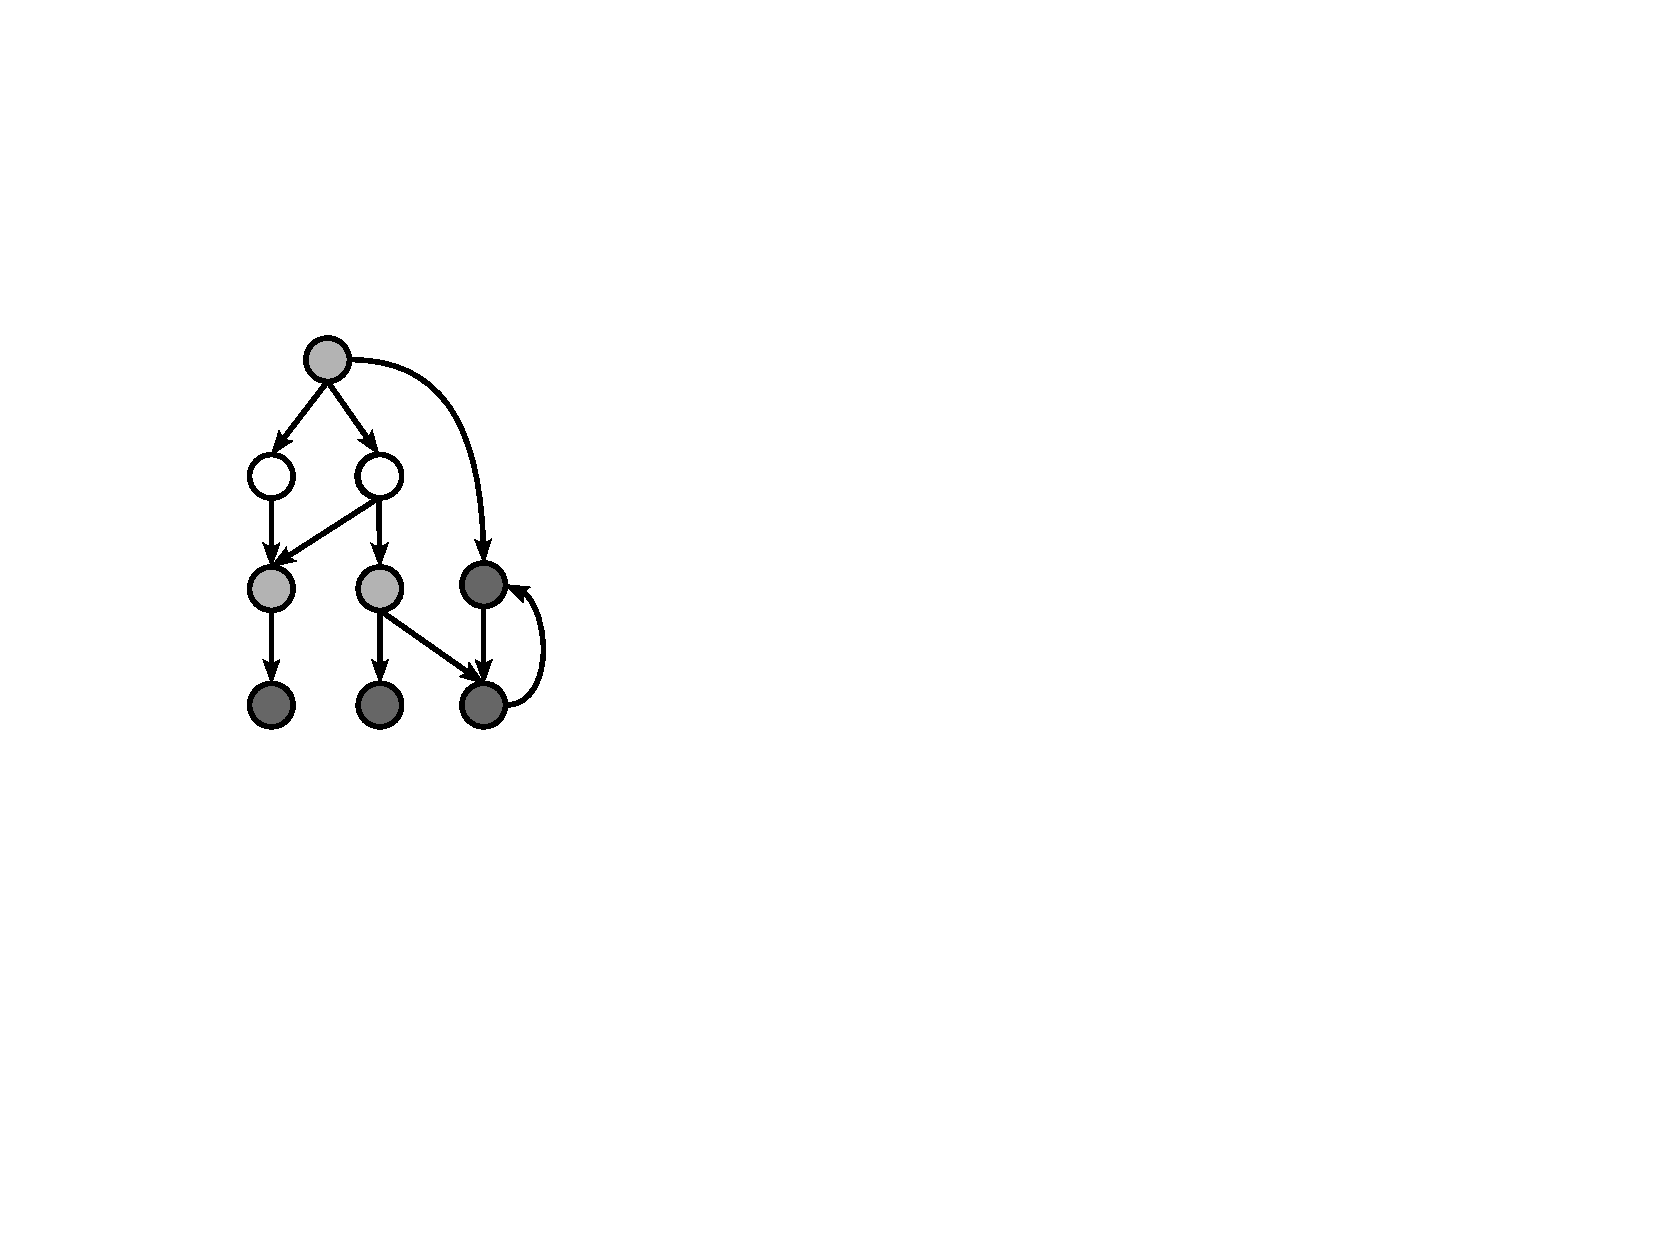
\includegraphics[width=0.3\textwidth]{part4/Figures/exampleGraph}
	\\ \vspace{5mm}
	}
}
\begin{subfloat}
\label{fig:graph-interfaces}
\begin{minipage}[b]{0.65\textwidth}
\begin{shortlisting}
interface Graph {
	Set<Node> getNodes();
	Set<Edge> getEdges();
}
interface Node {
	Color getColor();
	List<Edge> getChildren();
	List<Edge> getParents();
}
interface Edge {
	Node getFrom();
	Node getTo();
}
enum Color {
	White, LightGray, DarkGray
}
\end{shortlisting}
\end{minipage}
\caption{Abstract data types for nodes and edges.}
\end{subfloat}
	\caption{An example generic graph of three colors of nodes.}
	\label{fig:exampleGraph}
\end{figure}

\begin{figure}
\centering
\begin{subfloat}
\begin{minipage}[b]{0.44\textwidth}
\begin{shortlisting}
class Node {
   Color color;
   List<Edge> parent;
   List<Edge> child1;
   List<Edge> child2;
}
\end{shortlisting}
\end{minipage}
\caption{Concrete classes}
\end{subfloat}
\begin{subfloat}
\begin{minipage}[b]{0.568\textwidth}
\begin{shortlisting}
public Node(Color color) {
   color = color;
   parents = new ArrayList();
   children = new ArrayList();
}
\end{shortlisting}
\end{minipage}
\caption{Node constructor that uses the default \class{ArrayList} constructor.}
\label{fig:node-obvious-constructor}
\end{subfloat}
\caption{A straightforward implementation of the Node interface.}
\label{fig:node-obvious-impl}
\end{figure}

\autoref{fig:graph-interfaces} shows the interfaces for a \class{Graph},
\class{Node}, and \class{Edge} that one must implement. A common implementation
strategy, applied to the \class{Node} and \class{Edge} data types, is a
straightforward mapping of interfaces to concrete classes.
\autoref{fig:node-obvious-impl} shows such an implementation for the
\class{Node} data type. Following this
strategy, the \class{Node} class has three fields, to store its \class{Color}
and the relations to children and parents; these relations are implemented with a
standard collection, likely an \class{ArrayList}. The \class{Edge} class has two
fields, to store pointers to the source and target nodes. This implementation is
easy to implement. It is also easy to maintain: changes to the interfaces can be
directly mapped to changes to the implementation, because the two are parallel
versions of each other. The nodes and edges, and relations between them, are
objects that can be manipulated using normal object oriented practices; e.g. you
can write \texttt{node.getChildren().get(5).getTo()\-.getColor()}, which reads
as a fairly natural, albeit verbose, expression of what you intend.

\paragraph{A Straightforward Implementation}
Without any thought for memory concerns, the constructor for a node would be as
shown in \autoref{fig:node-obvious-constructor}. In this implementation, the
memory cost per node is three pointers plus two collections of default size. As
\autoref{tab:collection-costs} shows, the the default constructor of an
\class{ArrayList} allocates an array to hold 10 elements; the per-collection cost
is 80 bytes and the per-entry cost is 4 bytes. If no node has more than 10
parents or 10 children, then each node will consume one object header plus $3*4 +
2*(80 + 10*4)$, or $264$ bytes. If, on average, a node has one parent and 2
children, then 68 bytes (27\%) of this cost is wasted on null pointers. The 80
bytes (31\%) spent on the parent collection is unnecessary, for those nodes that
have exactly one parent. Even an optimally structured list which includes just
one pointer for a list with one entry would still impose two pointer costs to
reference a single parent node (one pointer to reference the list, one for the
list to reference the parent node).

In addition to the cost of the nodes are the cost of the edges objects. By
objectifying each edge, this implementation pays a cost of one object header
plus two pointers, or 24 bytes (20 bytes, before rounding up to an 8-byte
alignment boundary). For the example with an average of one parent and two
children per node, the effective cost per node is $264 + 3*24$, or $336$ bytes.

Ideally, a node with one parent and two children should consume four pointers, or
16 bytes: one to reference a \class{Color}, one to reference the parent node, and
two pointers to reference the children. The disparity between this optimal value
and the cost of the standard implementation is 320 bytes. A inspection of
\autoref{fig:maxActualData} shows that this implementation, with 16 bytes of
actual data and 320 bytes of overhead, can support at most 2.7 million nodes per
gigabyte of heap. An ideal implementation, with no storage costs beyond the
necessary 16 bytes of pointers, would be able to support at most 65 million nodes
per gigabyte of heap.

\paragraph{Optimizing the Implementation}
By specializing your code to handle only a limited degree of functionality, you
can achieve a fair degree of compactness without much effort. If every node has
exactly the same number of incoming and outgoing edges, an easy alternative
implementation presents itself. You can specialize the implementation for this
structural special case, and thereby eliminate the waste that comes from allowing
a flexible number of incident edges.
\autoref{fig:node-tuned-impls}a shows an implementation of the \class{Node}
interface that does away with collections. On top of the ideal implementation,
the cost per node is one object header plus two pointers for each of the three
\class{Edge} objects. On top of the 16 byte ideal cost, this implementation costs
an additional $3*(2*12 + 2*4)$ bytes, for a total of 112 bytes. This cost is one
third that of the initial implementation, though 7 times the cost of the ideal
implementation. This implementation supports just over 9 million nodes per
gigabyte of heap.

Even if many nodes have no parents, or fewer than two children, this specialized
implementation remains preferable to the original one that uses collections. This
is because an empty collection consumes no less than then the one pointer that
this collection-free implementation costs; this is the case if you point to the
singleton \code{Collections.emptyList()}. In the case when a node has one child,
then a list must be allocated, whose expense, even if the list has only a single
entry, will always be higher than a single pointer.

\begin{figure}
\centering
\begin{subfloat}
\begin{minipage}[b]{0.38\textwidth}
\begin{shortlisting}
class Node {
   Color color;
   Edge parent;
   Edge child1;
   Edge child2;
}
\end{shortlisting}
\end{minipage}
\label{fig:node-no-collections}
\caption{No collections}
\end{subfloat}
\qquad
\begin{subfloat}
\begin{minipage}[b]{0.38\textwidth}
\begin{shortlisting}
class Node {
   Color color;
   Node parent;
   Node child1;
   Node child2;
}
\end{shortlisting} 
\end{minipage}
\caption{No objectified Edges}
\label{fig:node-no-Edge-objects}
\end{subfloat}
\caption{Two implementations that have been specialized for the case where
no object has more than one parent and no more than two children.}
\label{fig:node-tuned-impls}
\end{figure} 

\autoref{fig:node-tuned-impls}b shows a yet more highly optimized \class{Node}
implementation that stores pointers to \class{Node}s, rather than \class{Edge}s.
One somewhat extreme variant of this implementation does not store \class{Edge}
objects at all. This \class{Edge}-free implementation approaches the ideal
implementation, in its capacity for storing large graphs. You must still pay one
object header per node, for the \class{Node} objects themselves. Thus, this
impementation has a per-node memory cost of 16 bytes for the pointers plus 12
bytes for the header. At this unit cost, a one gigabyte heap would support at
most 38 million nodes.

Though quite scalable, this implementation presents several complications. First
is the obvious limitation to at most one parent and at most two children per
node. Second, an \class{Edge}-free storage strategy dictates that the
\class{Node} API also be updated so that \code{Node.getChildren()} and
\code{getParents()} return a list of nodes, rather than a list of edges. You
cannot avoid storing \class{Edge} objects and yet support an external interface
of \class{Edge}s The same issue holds for an implementation that stores only a
single parent pointer: how can one efficiently support an interface that expects
a list of edges, if the storage contains only a single pointer? If you don't make
this API change, and instead choose to return facades that route the edge
operations properly, users of the API will be in for some surprises. The
following implementation does not work:
\begin{shortlisting}
public List<Edge> getParent() {
   List<Edge> list = new ArrayList<Edge>();
   list.add(parent);
   return list;
}
\end{shortlisting}
This implementation will not reflect any updates that the caller makes to the
returned list. It also violates the implicit reference-equality contract of
interfaces in Java: two calls to the \code{getParents()} interface must have
reference, i.e. \code{==}, equality. If possible, you can update
the written specification for the interface to indicate that a read-only
\emph{copy} of the parent list is returned. Unforunately, neither of these
policies can be statically enforced, and are hence prone to misuse.
Worse, if the interface design is out of the
scope of changes you can make, then you are out of luck and must cache the
returned list somewhere, so as to preserve reference equality.

Third, in addition to being quite expensive, in creating a list for every call to
\code{getParent}, this implementation lacks in expressive power compared to the
other implementations presented so far. For example you will find it more
difficult to extend the graph interface to support edge labels. Adding edge
labels with low overhead is not impossible, but requires some careful planning,
and thinking outside the Java box.

\paragraph{Difficulties of Supporting Edge Properties in Optimized
Implementations} If the API method \code{Node.getChildren()} returns a list of
nodes, rather than a list of edges, then the code to access an edge label of the
second child of a node can no longer be
\texttt{node.getChildren().\-get(1).getLabel()}. This way of traversing the graph
leads to a node, not an edge! Instead, edge labels must be fetched from some
larger entity, such as the graph model itself: e.g. \texttt{graph.getEdge(from,
to).getLabel()}, or \texttt{graph.getEdgeLabel(from, to)}. Without some care,
every edge label query will require a hash table lookup. Your design necessitates
storing the edge labels in a side data structure, one whose elements are not
directly connected, via pointers, to the nodes.

Storing edge labels in a parallel map-like structure makes sense only if a small
fraction of the edges have labels. Otherwise, the costs of the map infrastructure
may very well overwhelm the cost of the labels. Let's say that each label
consumes 4 bytes of actual data. A quick look at
\autoref{tab:collection-costs} shows that the per-entry cost of a \class{HashMap}
is 28 bytes. If, without edge labels, your implementation supports 38 million
nodes per gigabyte of heap (recall that this implementation supports at most
one parent and two children per node)
% 38 million is 16 bytes of data plus 12 bytes of header per node
then adding edge labels, in an ideal fashion that adds no additional overhead,
will decrease your capacity to 26.8 million nodes per gigabyte --- a reduction
in capacity of 30\%.
% 33.5 million is 16 + 12 + 4 bytes per node
If you store them in a \class{HashMap}, your capacity will decrease to at most
10.3 million nodes per gigabyte: the map costs 28 bytes per entry,
plus you need to create some sort of \class{Pair} object to house the source and
target nodes that form the map's key, plus you need to create a wrapper object to
house the edge label itself.
% 16 of actual data plus 12 bytes of header for the node 12+4+4 for the edges 4
% of actual data for the edge label 28 for the $Entry 12+4 for the Value 12+4+4
% for the Key
In contrast to the 30\% reduction of an ideal implementation of edge labels,
this straightforward implementation results in a 73\% reduction in capacity. In
this case the penalty of using a map is especially high because the starting
implementation, i.e. one supporting 38 million nodes per gigabyte, was fairly
highly tuned. The more highly tuned your memory design, the larger the negative
repercussions of subsequent bad choices. For example, if your starting
implementation supported 22 million nodes per gigabyte, then the penalty of a
map-based implementation of edge labels would be a somewhat lower 61\%.

A more efficient approach, if you have the luxury of modifying the \class{Node}
implementation directly, or subclassing it and overriding factory methods, is to
inline the edge labels directly into the \class{Node} class:
\begin{shortlisting}
class Node {
   Color color;
   Node parent;
   Node child1;
   Node child2;
   Label parentLabel;
   Label child1Label;
   Label child2Label;
}
\end{shortlisting} 
To avoid any need to maps, though, would require you to update the API for
fetching edge labels. Calling \code{graph.getEdge(from, to).getLabel()} with
this implementation would require an intervening map structure. In contrast,
an API that had the form \code{node.getParentLabel(0)} and
\code{node.getChildLabel(1)} would allow for direct access to the labels,
without a map. Inlining the storage for labels requires a concomitant inlining
of the APIs. Therefore, while this implementation
approaches the optimal capacity, it is not especially desirable, from an
engineering perspective.
 
\paragraph{Insufficiencies of Pure Object Orientation}
This activity of tuning the original graph implementation has lead to two
difficult ends. First, it is difficul to support nodes with widely
varying numbers of parents and children. If all nodes had only a very small number of incident
edges, or a very large number, then specialized implementations are possible.
Second, optimizing storage has come at the expense of easy extensibility; one
can remove the use of \class{Edge} objects, but, to support edge labels 
requires either expensive maps to parallel data structures, or 
pollution of data types not directly connected to the planned extension.

Using a fully object-oriented Java design, it is impossible to achieve both
compactness of storage and the generality to handle a variety of graph
structures. To do so requires coding in a style that is not conventionally object
oriented.



% Shortly, we will discuss the
%complexities, but benefits, of the latter style of API.




\section{Breaking the Mold of Object Orientation}
\label{sec:fortran-style}

The examples of the previous section worked through various optimizations of
representing relationships, and illustrated the interplay of storage optimization
and API design. Very often, achieving a high level of memory efficiency requires
breaking what would generally considered to be the object orientation of the API
or the storage. The main goals are to support a combination of flexibility and
scalability that is not possible when following the precepts of object
orientation.

\subsection{Supporting Singleton Sets}

% If the distribution of the sizes of these sets is starkly bimodal, where most
% of the sets are either fairly large, or

One common case, when using collections, is that many of them contain zero or
only a single element. It seems silly to pay the expense of a full-fledged
collection for these special cases. The Java standard library offers has a
partial solution to the case of many empty collections, in the form of the family
of factor methods that include \code{Collections.emptySet()} and
\code{Collections.emptyList()}.
\index{Empty Collections}
These are partial solutions, because they only handle the case of unchanging
collections. There is no provision, in the standard libraries, for optimized
storage of single-entry collections. Consider our graph from the previous
section:
\begin{shortlisting}
class Node {
	Color color;
	List<Edge> parents;
	List<Edge> children;
}
\end{shortlisting}
The previous section proposed an optimization for the special case of nodes with
at most one parent. If this were always the case, for every single node ever
created by your application, then it is valid, and indeed a good idea,
to change the \class{Node} class definition to inline the pointer to that
potential part. If it is only sometimes the case, then this trick does not work.

You can regain a degree of flexibility, at the expense of some added coding
complexity. First, you must update the \class{Edge} interface to indicate that an
edge is also capable of acting as a singleton list of edges:
\begin{shortlisting}
interface Edge extends List<Edge> {
}
\end{shortlisting}
Second, you must update your edge implementations to implement the boilerplate of
the \class{List<Edge>} interface; this part is straightforward. It then becomes
possible to have a single node implementation that supports arbitrary numbers of
parents, but is also optimized the special case of nodes with only a single
parent. This is possible, without your having to change the fields of the
\class{Node} class in any way. The final change you need to make 


By specifying that the parents of a node are a \class{List<Edge>},
you are forced to 

\subsection{Bulk Sharing of Immutable Data}
\label{sec:bulk-sharing-pool}

Primitive arrays are often the repository for most of your application's actual
data. If your application has a few large primitive arrays, then the overhead of
the arrays will be dwarfed by the actual data contained therein. A common problem
with Java applications is that they have many small primitive arrays.
\index{Small Primitive Arrays} If the large majority of your actual data is in
these primitive arrays, and the average length of each array is 10 characters,
then your application will have a memory bloat factor of 61\%
% 16/(10 + 16)
--- almost half of your heap will be wasted on the object headers of the
primitive arrays. The problem grows worse if these primitive arrays are wrapped
inside of objects such as \class{String} or \class{ByteArrayOutputStream}. If
wrapped inside of \class{String} objects, then your application is doomed to a
memory bloat factor of 83\%.
% (16+32)/(10+16+32)

If these primitive arrays store only a small number of distinct sequences, this
problem of high overhead can, at least indirectly, be addressed by
interning.\index{Interning} Earlier, \autoref{sec:sharing-strings} discussed
string interning. If your primitive data is string data, then you can use the
\jres built-in mechansm for pooling this data, so that only one copy of each
string is kept in memory. For non-string data, you will have to roll your own
solution. In any case, however, interning only tackles a part of the problem at
hand. By keeping only a single canonical copy of the primitive data, you
eliminate the primitive array headers for the duplicates.
\autoref{fig:bulk-sharing-pool}a and \autoref{fig:bulk-sharing-pool}b illustrate
a simple case of interning. Of three strings, there are two duplicate ``grape''
sequences. The residual high overhead is due to the remaining primitive array
object headers, and all of the \class{String} objects; none of the \class{String}
objects are eliminated by interning. Interning removes only the duplicate
primitive array overheads.


\begin{figure}
\centering
	\subfigure[Three normal	\class{Strings}.]{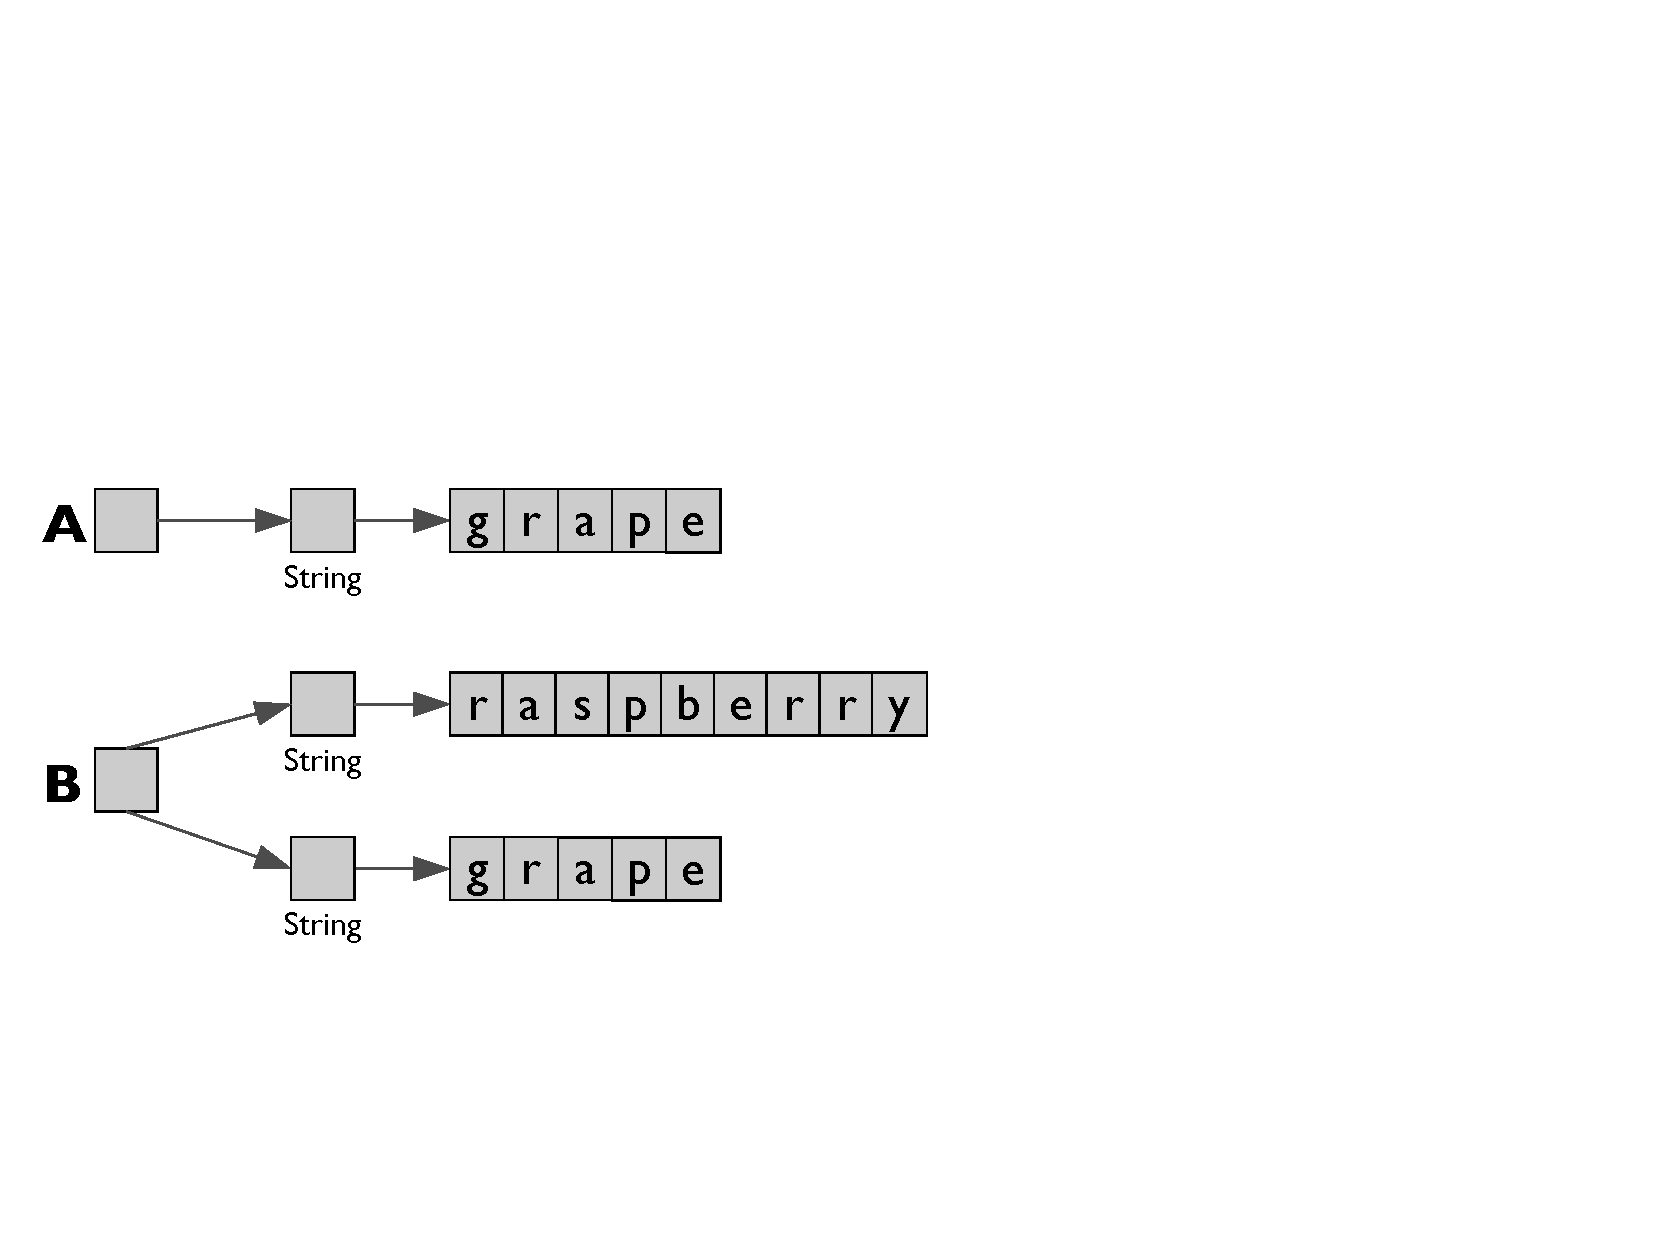
\includegraphics[width=0.425\textwidth]{part4/Figures/bulksharingpool1}}
	\qquad
	\subfigure[Interning.]{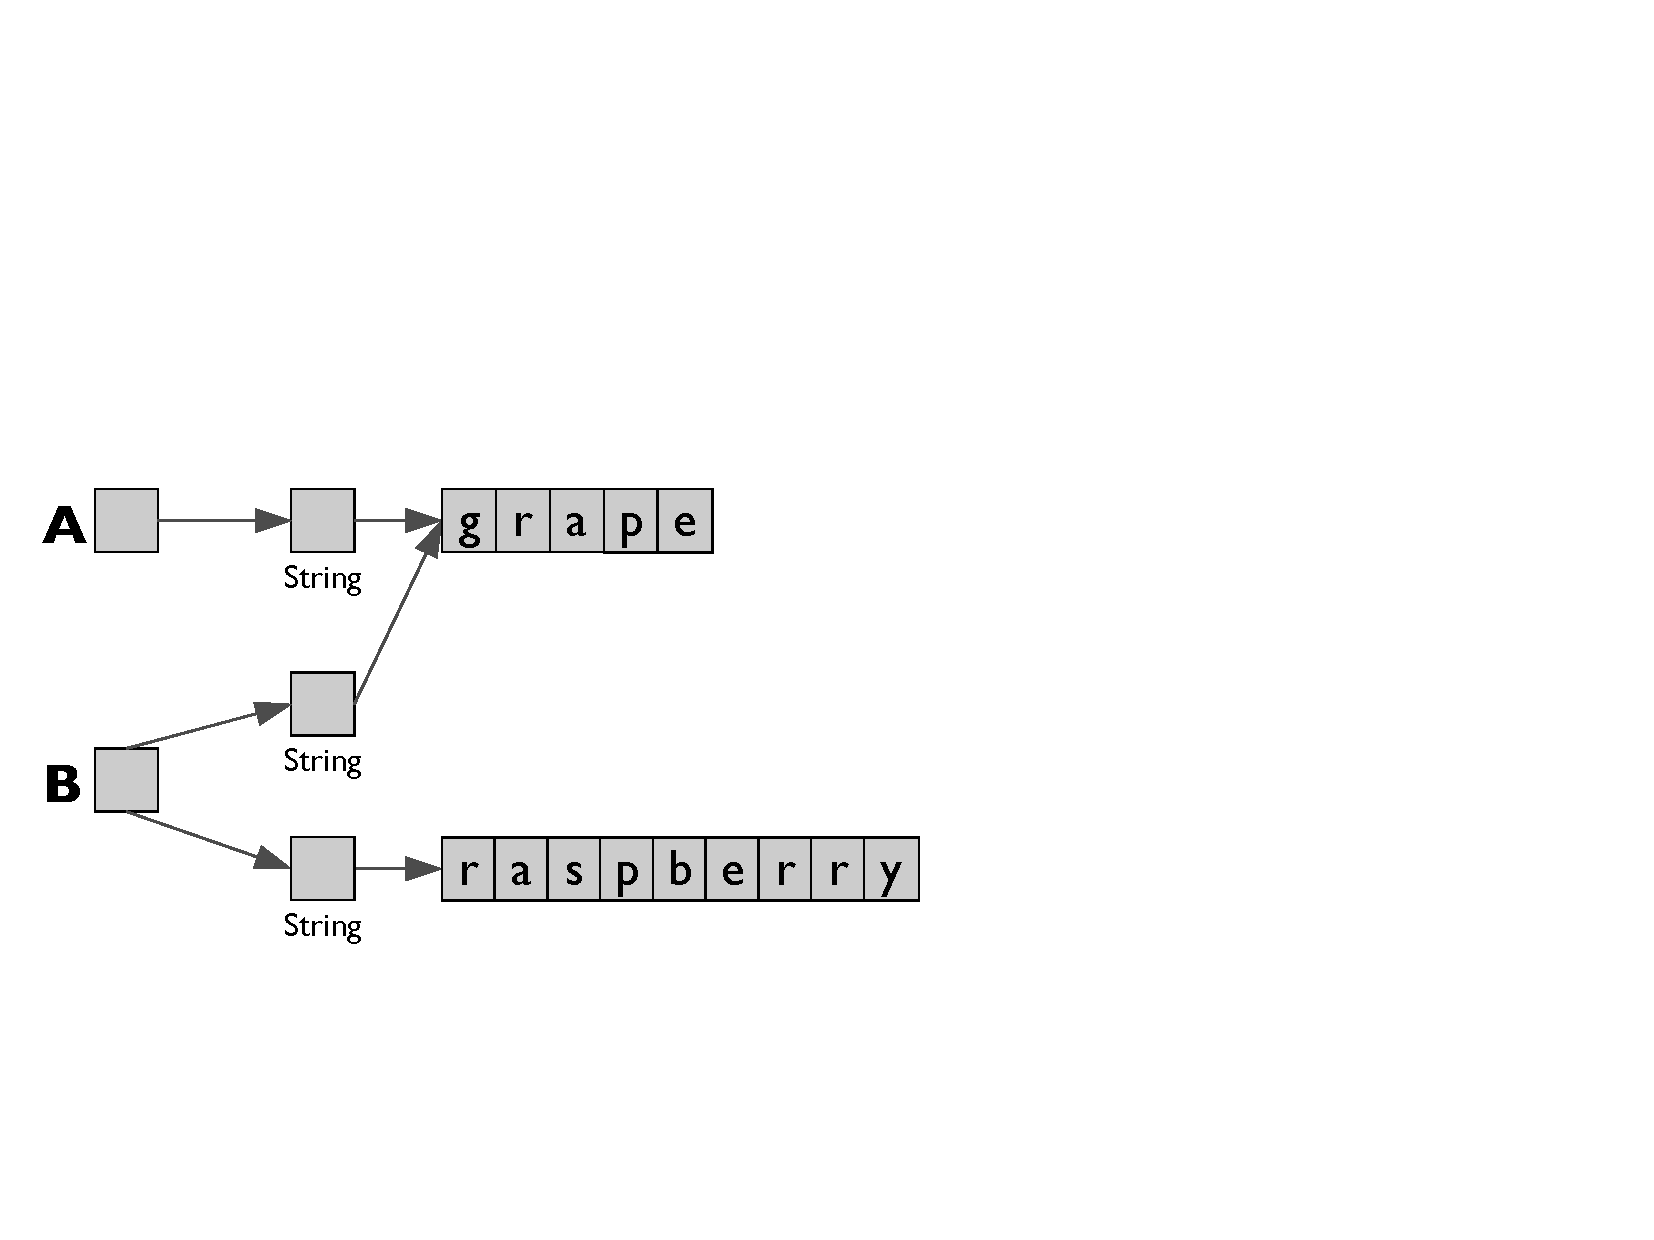
\includegraphics[width=0.425\textwidth]{part4/Figures/bulksharingpool2}}
	\qquad
	\subfigure[Bulk	sharing	pool.]{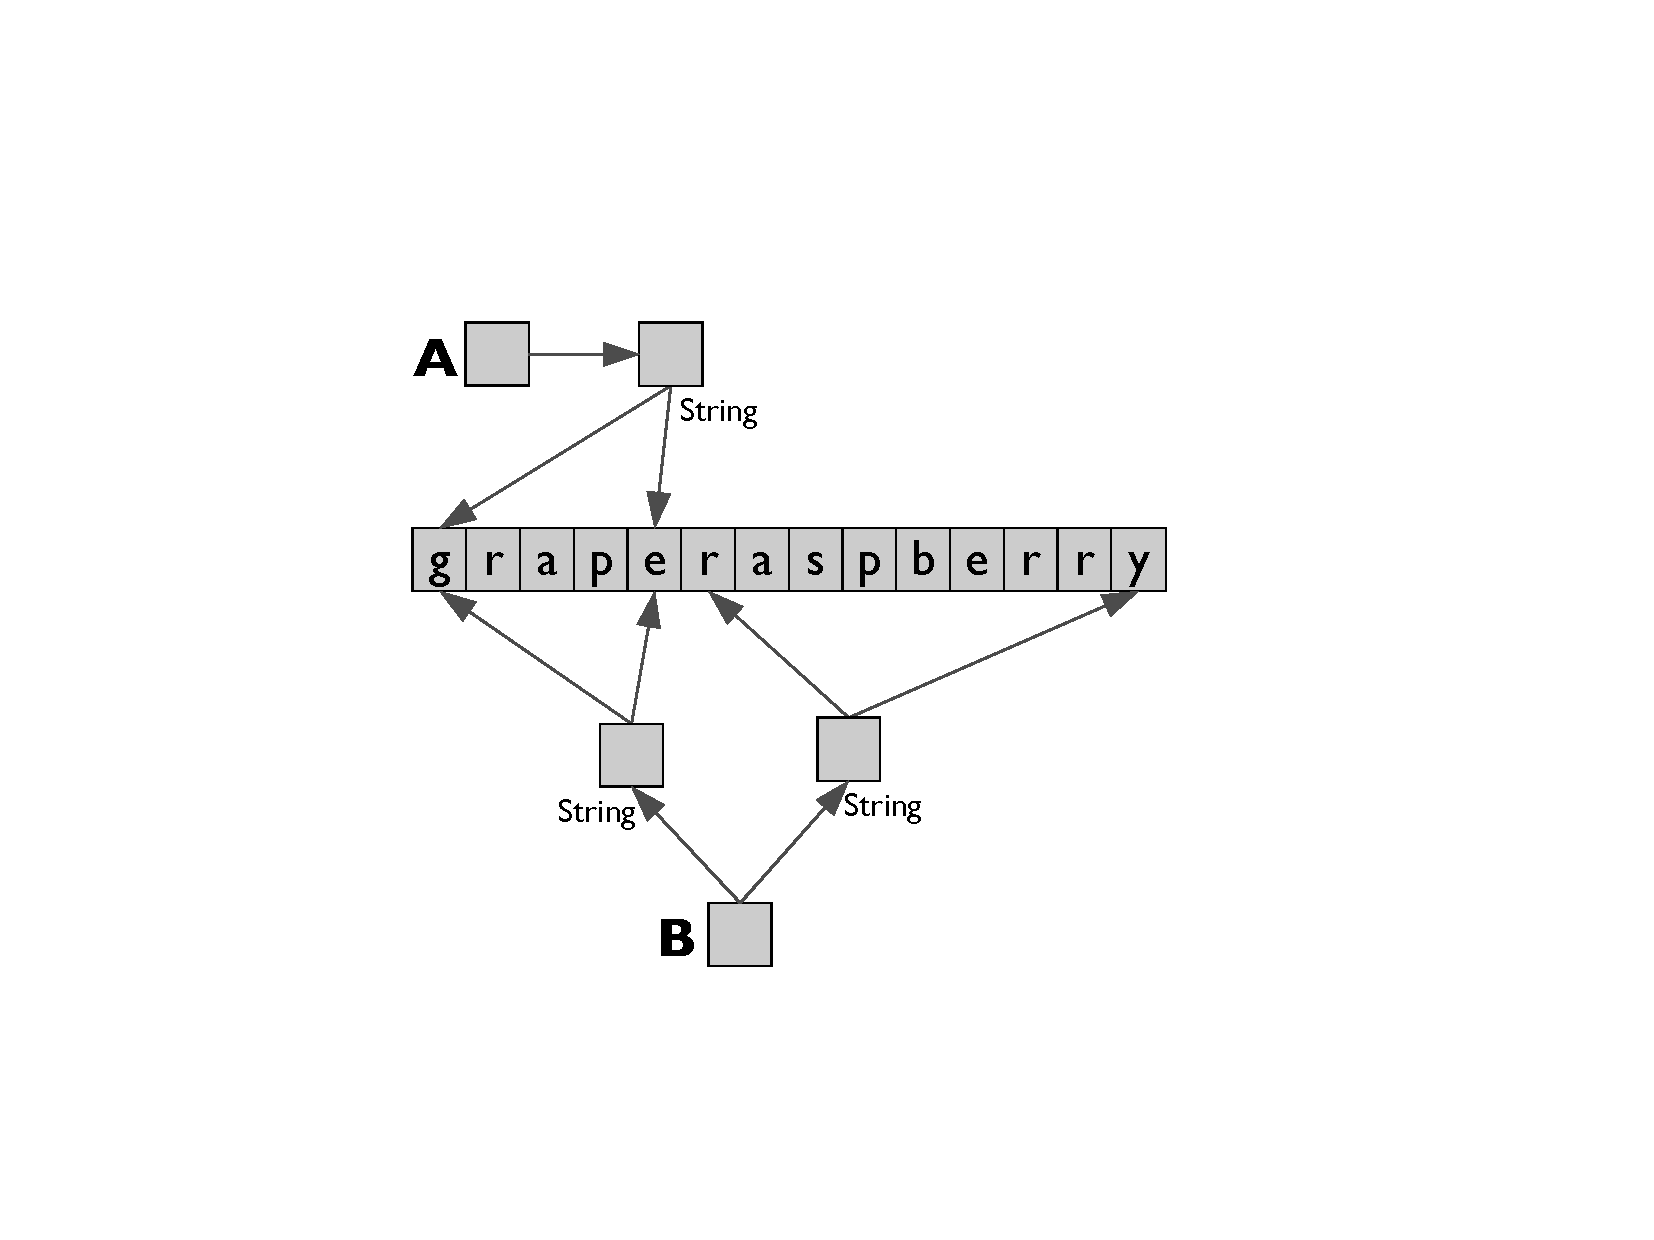
\includegraphics[width=0.36\textwidth]{part4/Figures/bulksharingpool3}}
	\qquad
	\subfigure[Bulk	sharing	pool, no wrappers.]{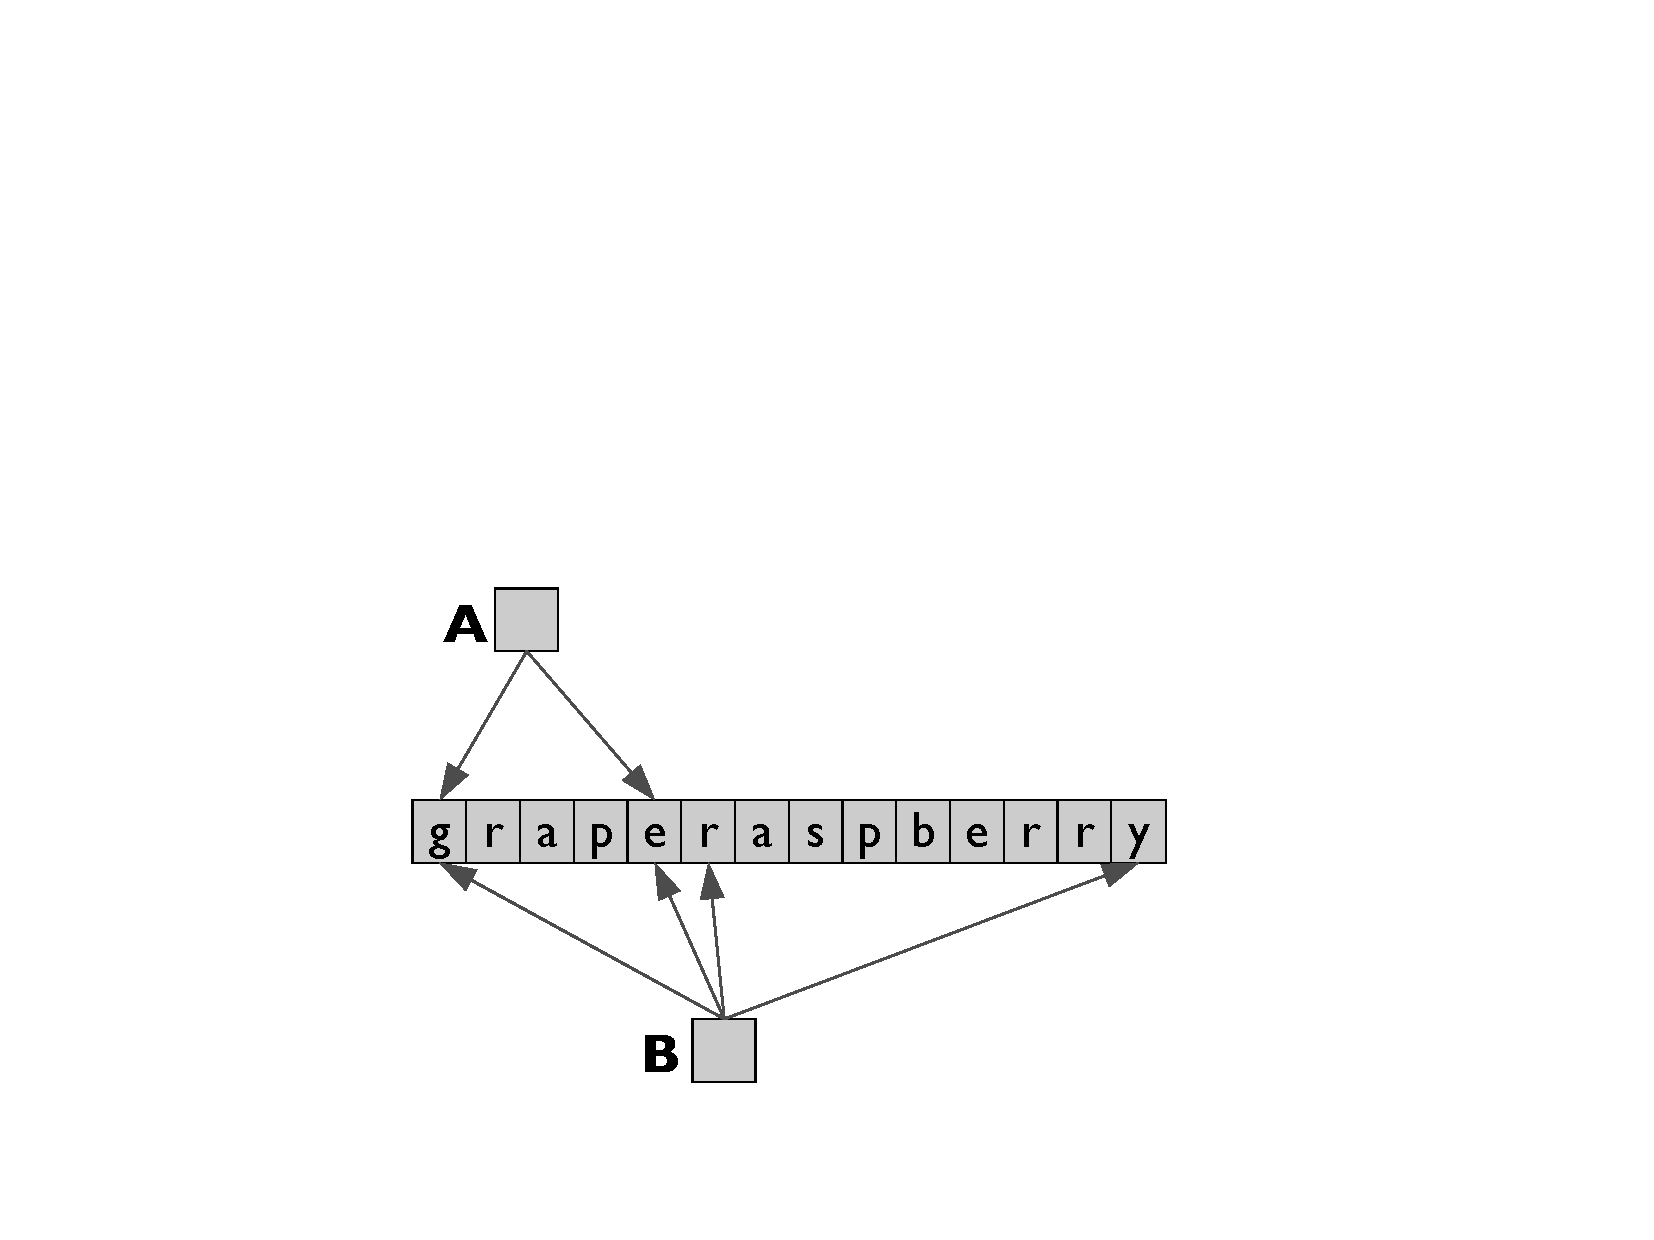
\includegraphics[width=0.36\textwidth]{part4/Figures/bulksharingpool4}}
	\subfigure[The memory consumed by one million strings, each of length 10
	bytes, for varying degrees degrees of distinctness; e.g. 10\% means that
	there are only 100,000 distinct strings.]{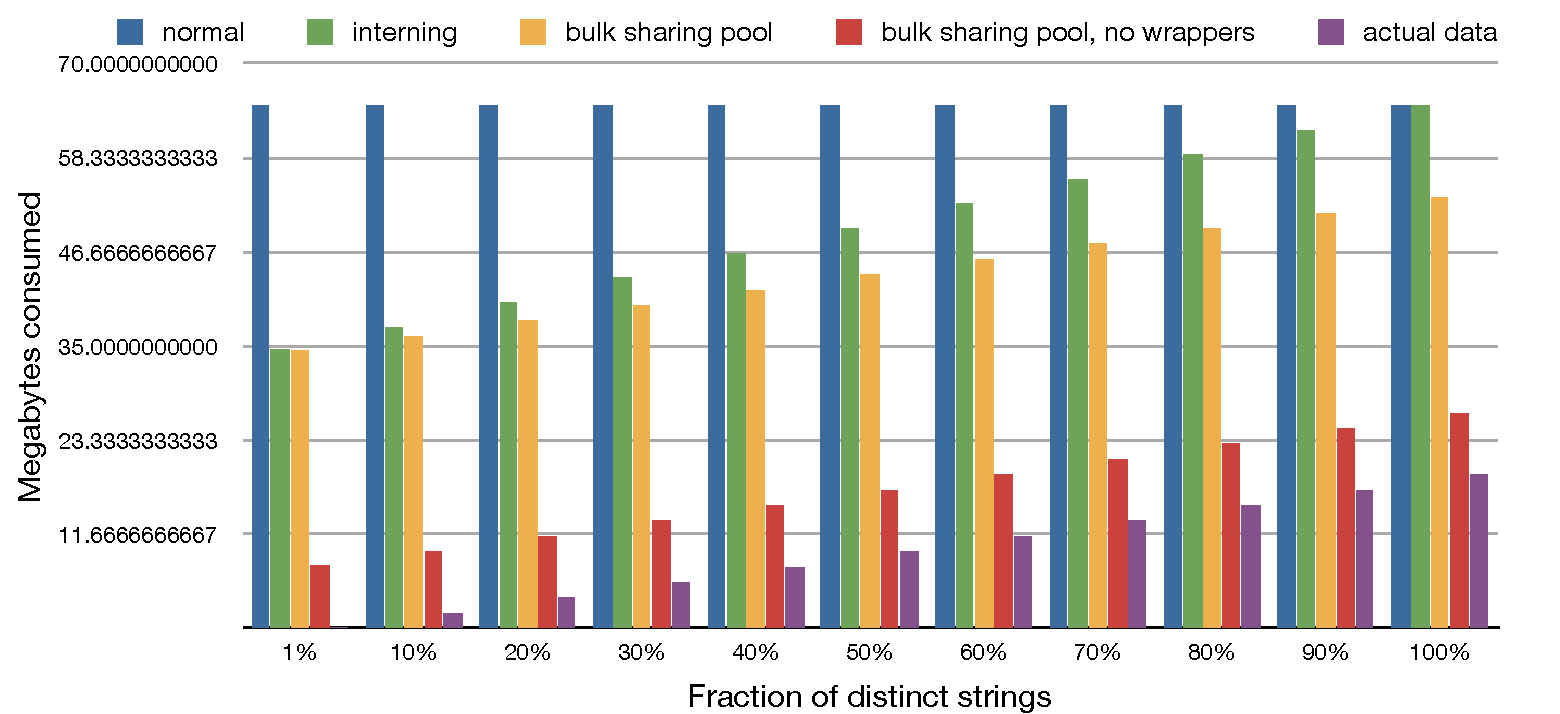
\includegraphics[width=\textwidth]{part4/Figures/bulksharingpool_consumptionchart.pdf}}
	\caption{If your application has many long-lived, but small, arrays of
	primitive data, it could suffer from high overhead. Interning avoids
	duplication. On top of interning, a Bulk Sharing Pool offers the additional
	potential for you to eliminate the primitive array wrappers, and so can be
	beneficial if there are still a large number of unique sequences.}
	\label{fig:bulk-sharing-pool}
\end{figure}

By eliminating many duplicates via interning, you stand to save a large amount of
memory, but your memory bloat factor will still be quite high. Instead of a bloat
factor of 83\%, with interning your heap will have a bloat factor of at least
88\%.
% 3*(16+32)/(10*2+3*(16+32))
This value is a lower bound, because there is another curious problem that arises
when handling duplicate data. If there is a bounded number of distinct sequences,
but an increasingly large number of total sequences, your memory bloat factor can
approach 100\%. In this case, the per-sequence memory overhead grows with the
number of sequences, but the amount of actual data is bounded by the number of
distinct sequences.

There are two further optimizations open to you, but these require deeper
changes. Both optimizations store all of the sequences in a single, large array.
This storage style is an example of optimizing for a bulk of uniformly typed data
that is accessed in a uniform, and stylized, fashion. Why pay the expense of many
small primitive arrays, if your code does not need each sequence to be a Java
object? If you will never synchronize or reflect on sequences, as objects, then
the primitive array header is a needless expense.
\autoref{fig:bulk-sharing-pool}c illustrates this bulk storage of the sequences
in a single large array. You pay the primitive array overhead just once, across
all pooled sequences, rather than for every sequence. 
%In this case, your heap
%will have a memory bloat factor of
% 3*(16+32)/(10*2+3*(16+32))

To achieve the ultimate in memory efficiency, you must also eliminate the
\class{String} wrapper objects. This last step requires the most work on your
part. If you have the luxury of modifying the class definitions for the objects
that contain the string wrappers, then you can replace every pointer to a string
with two numbers. These numbers store indices into the single large
array of bulk data, and demark the sequence that the string wrapper would have
contained. You are essentially inlining the offset and length fields that every
Java \class{String} object has, and doing away with the hashcode field and the
extra header and pointers. This eliminates almost all sources of overhead.

\autoref{fig:bulk-sharing-pool}d charts the memory consumption of the four
implementations: using normal Java \class{Strings} without any attempt to remove
duplicates; using Java's built-in string interning mechiansm; using a bulk
sharing pool; and using a bulk sharing pool without any \class{String} wrappers.
The chart also includes a series comparison with the amount of memory consumed by
actual data.  The chart shows memory consumption of each implementation for
varying degrees of distinctness of the strings, for an case with one million
strings of length 10 characters each.
For example, if 500 thousand of the million strings are distinct (which
corresponds to the 50\% point in the chart), the normal implementation consumes
65 megabytes, the interning implementation consumes 50 megabytes, the bulk
sharing pool implementation consumes 44 megabytes, and the bulk implementation
without string wrappers consumes 17 megabytes. There are 500 thousand
distinct characters, so the actual data consumes about 10 megabytes.

\subsection{Column-oriented Storage}
\label{sec:column-oriented}

\section{Memory Mapping and Marshalling}